% This is samplepaper.tex, a sample chapter demonstrating the
% LLNCS macro package for Springer Computer Science proceedings;
% Version 2.20 of 2017/10/04
%
\documentclass[runningheads]{llncs}
%
\usepackage{graphicx}
\usepackage{tabularx}
% Used for displaying a sample figure. If possible, figure files should
% be included in EPS format.
\usepackage{float}
\usepackage{enumerate}
%
% If you use the hyperref package, please uncomment the following line
% to display URLs in blue roman font according to Springer's eBook style:
%  \renewcommand\UrlFont{\color{blue}\rmfamily}
\raggedbottom
\begin{document}
%
\title{QALD-Mini-Project}
%
%\titlerunning{Abbreviated paper title}
% If the paper title is too long for the running head, you can set
% an abbreviated paper title here
\newcolumntype{Y}{>{\centering\arraybackslash}X}
\newcommand\tab[1][1cm]{\hspace*{#1}}
\author{Lukas Bl{\"u}baum \and
Nick D{\"u}sterhus \and
Ralf Keller}
%
\authorrunning{L. Bl{\"u}baum, N. D{\"u}sterhus et al.}
% First names are abbreviated in the running head.
% If there are more than two authors, 'et al.' is used.
%
\institute{University of Paderborn ,Warburger Str. 100, 33098 Paderborn, Germany
\email{\{lukasbl,nduester,rkeller\}@uni-paderborn.de}
\url{https://github.com/LukasBluebaum/QALD-Mini-Project}}



%
\maketitle              % typeset the header of the contribution
%
\begin{abstract}
As part of the lecture "Semantic Web", we developed a template based Question answering engine. The Question answering engine is able to answer different types of questions using DBpedia as the knowledge base to extract those answers.
The engine maps keywords to find information that are needed to generate appropriate SPARQL queries. Including keywords that are used to determine the selection of the templates.
Those information can be properties and classes. DBpedia Spotlight is used to find the entities of the questions.
We iterate over the set of information needed to fill in the templates.
The properties get ranked, to improve the probability that our first query returns a correct answer.
Our engine achieves an F-score of 0.527 for the QALD8-Test Dataset.

\keywords{QALD  \and Question Answering \and Spotlight \and SPARQL.}
\end{abstract}
%
%
%
\section{Introduction}  

The World Wide Web is filled with information for everyone to explore. Most information on the Web is unstructured, what makes it hard to process for humans and computers. The Semantic Web is a approach to provide structured data in the Web that is easy to process by computers and can be processed to be easily understood by humans. \\

Most Semantic Web Databases use SPARQL as the language to query the database. That means that in order to search the semantic web the user has to learn a query language, that is not very easy to learn. This is not user friendly and can be improved. \\

The goal of our project is to provide a interface that takes a question formulated in natural language and answers it by querying DBPedia. The interface will be able to be used over the web via HTTP-POST requests. We aim for a F-measure of at least 0.1. \\

Our project uses a Template-based approach. That means we have defined templates of SPARQL-Queries that are modified at predefined locations based on the question asked. The project consists of three components: The \emph{Question-Answering (QA) Engine}, the \emph{Question-Processor} and the \emph{SPARQLQueryBuilder}. We use the Library \emph{qa.annotation} to find entities, properties and classes, qa.commons to load and store QALD-datasets and GERBIL QA, a wrapper for web communication. \\

The \emph{QA Engine} is responsible for providing the interface to users. It reads questions from the Webservice or a predefined dataset and passes the question to the Question Processor. Furthermore the QA Engine is responsible for outputting the answer, i.e sending a HTTP-Response to the user. \\

Relevant entities contained in the question have to be identified and the question has to be analyzed to determine the type of the question. This is done by the \emph{Question Processor} component. \\

To get a answer a SPARQL-Query has to be build and executed on a endpoint. That is the responsibility of the \emph{SPARQLQueryBuilder}. This component uses the processed information provided by the Question Processor, builds a SPARQL-Query by using predefined templates and executes the query on an endpoint provided by DBPedia. \\ 

\pagebreak
\section{Simplified Procedure} 
\begin{figure}
	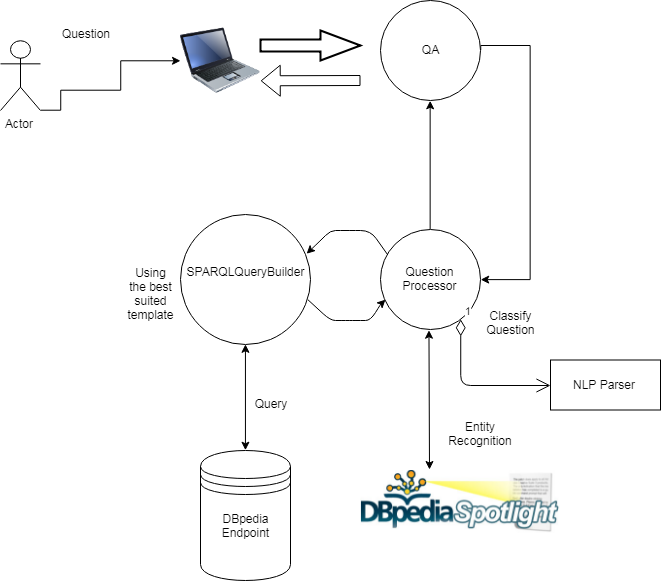
\includegraphics[width=\textwidth]{Architecture.PNG}
	
	\caption{Architecture.}
	\label{fig1} 
\end{figure}

The Question Answering processing includes multiple steps. After the question have been received, the question will be forwarded to the QuestionProcessor by the QA class. \\
This class annotates the questions with all additional information that are important to be able to find an answer. 
The question is sent to DBpedia Spotlight which performs named entity recognition. The found entities are saved in a question object. 
Following this, we use the Stanford CoreNLP \cite{stanford} in order to find words that could indicate which DBpedia property we will need to later fill in the templates. \\
Therefore we pass those keywords to  IndexDBO\_classes provided by the qa.annotation library. \\
Furthermore, the IndexDBO\_classes maps the nouns of the question to classes if a corresponding class exists in the DBpedia namespace. The IndexDBO class itself performs a fuzzy search on a predefined file that contains a set of DBpedia properties and keywords using the Apache Lucene library. \\
All gathered information will be stored in the question object. \\
Then we classify the question based on the question word ( cf. 5 Template overview). \\
Depending on the classification the SparqlQueryBuilder class, given the question object, runs a method in which a SPARQL template will be filled in with the found entities, classes and properties. \\
The method itself does some selection of which SPARQL template will be used out of some prepared templates - corresponding to the first classification - based on keywords ( e.g. many or comparatives) and the number of entities and classes. \\
Then we query the DBpedia SPARQL endpoint using apache Jena with all SPARQL queries that seem meaningful given the set of possible properties.
The result is returned and converted to an answer JSON object by the provided gerbil wrapper classes. \\


\section{QA System}

The QA-System component is the component that reads questions from various datasources and relays them to other components, mainly to the \emph{Question Processor}. It is also responsible for outputting the answer to asked questions. \\
	
There are three supported input-modes:  

\begin{enumerate}
	\item Ask a single question stored in a variable
	\item Load datasets with multiple questions from a JSON-File 
	\item Run a queryable webservice 
\end{enumerate}

Option 1 is mainly used for debugging purposes and is not of further interest. The second option is used to run practice datasets provided by the dice research group. Our aim of a F-Score of at least 0.1 refers to these datasets. Option 3 is used to provide a webservice a user can use to get their questions answered. \\

The QA-Component consists of multiple subcomponents. One subcomponent is the \emph{QA} class. This class is the main class of the program, the \emph{main} Method is invoked on startup. It is responsible for checking which mode the program should run in. The mode is defined by a flag in the code that has to be set at compile time. It loads the question and releys them to the Question Processor, based on which mode is selected. If the program runs in \emph{Dataset} mode, the QA class is also responsible for writing the results as a JSON-File to the local storage. To load the dataset, we use the \emph{LoaderController} class provided by the dice research group. \\

The second component is the \emph{QA-System} component. This class' only purpose is it to take a question and return a \emph{Answer Container}. The Answer Container contains the answer of the question and the query used to get the result. The QA-System relays the question to the QuestionProcessor to get the Answer Container. The QA-System is mainly used by the webserver to determine the answer to a given question. \\

\subsection{Webserver}

The third component is the webserver that listens for questions over HTTP. The webserver is part of the GerbilQA-Benchmarking-Template provided by the dice research group. It utilizes the Spring-Framework to provide the service over the web. \\

The webserver starts listening for HTTP-POST requests under the \emph{/gerbil} path. The parameter of the requests have to contain the question to be answered under the \emph{query} parameter and the language of the question under the \emph{lang} parameter. \\

The webserver relays the the question to the QuestionProcessor by using the \emph{QA-System} component, which returns an \emph{Answer Container}. The webserver converts the Container to a JSON-String, which is sent to the user as a response to their POST-request.

\section{Question Preprocessing} 
Before we can start to build a SPARQL-Query we need to preprocess the questions. First we classify them depending on their starting word, because by doing so we can already get many information about the expected answer. So for example if we have a "When" question we already know that the answer should be of datatype date or year. \\

Then we use the Stanford CoreNLP to find keywords inside the questions. Here we extract nouns, verbs and adjectives and later map them to classes and properties from the DBpedia ontology. We also extract superlatives and comparatives to further differentiate the used templates. For the Named Entity Recognition we request the Spotlight \cite{spotlight} demo through the qa.annotation library. Then we remove entities that can also be mapped to classes, because somtimes Spotlight detects something like "Mountain" also as entity (resource) and we normally want to use that as a class and not an entity. \\

Finally we apply the IndexDBO classes of the qa.annotation library to the extracted nouns,verbs and adjectives to map them to classes and properties from the DBpedia ontology. Here normally verbs, adjectives will be mapped
to properties and nouns to classes. In the next step we will then rank the properties, so that we can test the properties with the most hits, triples on DBpedia with that property, first. We also extented the property list in qa.annotations and just added all DBpedia ontology properties.

\section{Template Overview}
Below in table 1 you can see a quick overview of some of the question types we differentiated. Afterwards we also looked at the number of entites and classes and if there is a superlative or comparative to choose the template accordingly. Finally we requested the DBpedia endpoint using Apache Jena.

\begin{table}
	\caption{A quick overview for some of the question types.}\label{tab1}
	\begin{center}
		\begin{tabularx}{\textwidth}{@{}|Y|Y|@{}}
			\hline
			\textbf{Question type} &  \textbf{Expected answer} \\
			\hline
			boolean (Do, Did, Has, Was, Does ... ) &  true or false \\
			\hline
			Where &  Place \\
			\hline
			When &  datatypes date or year \\
			\hline
			Who &  Person \\
			\hline
			List, Name, Show ... &  list of resources \\
			\hline
		\end{tabularx}
	\end{center}
\end{table}

\subsection{Example}
An example for the most basic query consting of $<$entity$>$ $<$property$>$ ?answer.
\begin{example}
	"Who was the doctoral supervisor of Albert Einstein?"\end{example}
First we see that it is a "Who" question so we already know that the answer should be a Person.
Spotlight will find one entity: \textit{dbr:Albert Einstein}. Then \textit{doctoral supervisor} will be mapped to \textit{dbo:doctoralAdvisor}.

\begin{example}
	SELECT DISTINCT ?answer WHERE \{ \\
	\tab[1.8cm] ?answer a foaf:Person. \\
	\tab[1.8cm] $<$http://dbpedia.org/resource/Albert Einstein$>$ \\
	\tab[1.8cm] $<$http://dbpedia.org/ontology/doctoralAdvisor$>$ ?answer . \} \end{example}



\subsection{Superlatives, Comparatives} 

When the user enters a question like \emph{What is the highest mountain in Germany?}  the SPARQLQueryBuilder builds a query that fetches all mountains in Germany, sorts them descending by height and selects the first entry. This process is applicable for every other superlative and comparative. \\

The QueryBuilder has to know which superlatives and comparatives there are, which attributes they compare and if the result has to be descending or ascending. There is no online resource which provides this information, so we created an Enum called \emph{Comparisons} that contains a selection of superlatives and comparatives in connection with the corresponding sort order (ascending for lowest, smallest, descending for highest, longest) and a reference to appropriate DBPedia attributes. \\

The \emph{SPARQLQueryBuilder} iterates over all comparatives and superlatives and checks if the question contains any of them. If the Builder detects a comparative or superlative it selects the appropriate predefined Query-Template and modifies it according to the data saved in the enum. By using this approach we have a quick and uncomplicated way to handle comparatives and superlatives. The disadvantage of this approach is that we can only handle comparatives or superlatives that we defined on attributes we defined. If the user wants to compare an attribute we have not thought about this approach will not yield any result. See the table 2 below for a few example entries from the Comparison enum.

\begin{table}
	\caption{A few example entries from the Comparison enum.}\label{tab1}
	\begin{center}
		\begin{tabularx}{\textwidth}{@{}|Y|Y|Y|@{}}
			\hline
			\textbf{Word} &  \textbf{Uri} &  \textbf{Order}\\
			\hline
			largest &  dbo:areaTotal & DESC \\
			\hline
			tall &  dbo:height & - \\
			\hline
			taller &  dbo:height & DESC\\
			\hline
			tallest &  dbo:height & DESC\\
			\hline
			high &  dbo:elevation & - \\
			\hline
			higher &  dbo:elevation & DESC\\
			\hline
			highest &  dbo:elevation & DESC\\
			\hline
		\end{tabularx}
	\end{center}
\end{table}


\subsection{Example}
\begin{example}
	"What is the largest country in the world?"\end{example}
Here Spotlight will find no entity. We detect the class \textit{Country} and from our Comparison enum the word 
largest (dbo:areaTotal) with the order "DESC". 

\raggedbottom
\begin{example}
	SELECT DISTINCT ?answer WHERE \{ \\
	\tab[1.8cm] ?answer rdf:type $<$http://dbpedia.org/ontology/Country$>$. \\
	\tab[1.8cm] ?answer $<$http://dbpedia.org/ontology/areaTotal$>$ ?area . \} \\
	\tab[1.8cm]	ORDER BY DESC(?area) LIMIT 1 OFFSET 0\end{example}

\pagebreak
\section{Benchmarking and Evaluation} 

The GERBIL platform computes an F-score over our answers. We evalutated the QALD8\_Train as well as the QALD8\_Test set.

\begin{figure}[H]
	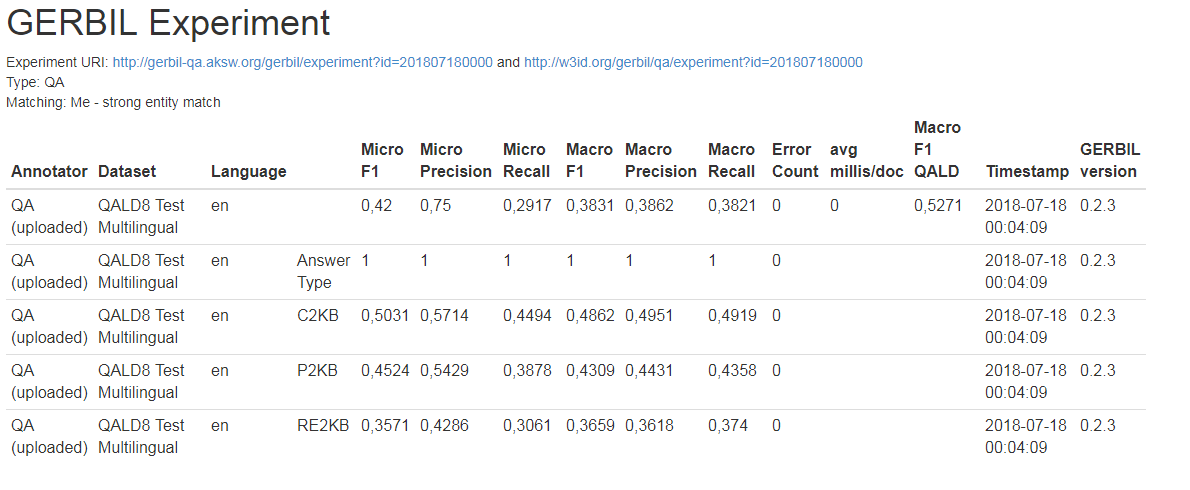
\includegraphics[width=\textwidth]{QALD-8-Test.PNG}
	 http://gerbil-qa.aksw.org/gerbil/experiment?id=201807180000
	\caption{Gerbil experiment for the QALD8-Test set, with a F-measure of 0.527.}
	\label{fig2} 
\end{figure}


\begin{figure}
	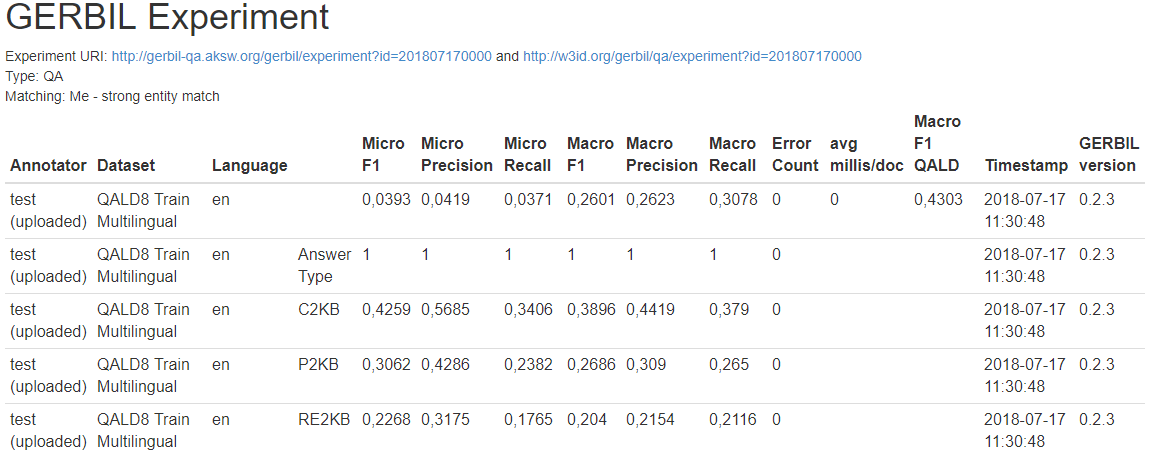
\includegraphics[width=\textwidth]{QALD-8-Train.PNG}
	
	 http://gerbil-qa.aksw.org/gerbil/experiment?id=201807180003
	\caption{Gerbil experiment for the QALD8-Train set, with a F-measure of 0.45.}
	\label{fig3} 
\end{figure}

\pagebreak
\section{Discussion} 
Our system reaches an F-score of about 0.527. This is partly due to the number of properties to which the words of the question can get matched to otherwise, some question that could be answered with a simple SPARQL query could not be answered. \\

Further factors include the ordering of those properties and a larger number of different templates. 
The QALD8 set has a focus on questions containing comparative, superlative as well as temporal aggregators, so our templates are mostly designed to answer those kinds of questions. \\

Presumably, our system will have a slightly worse result on other questions sets. For example the selection of templates for boolean and list questions could be improved.  Our system provides the foundations to answer a multitude of questions, so it could easily be extended to further improve the result.\\

Our system is not able to understand the semantics of the questions. \\
Nevertheless identifying keywords to map those to classes and properties as well as keywords that enable us to classify the questions leads to an appropriate selection of a SPARQL-Query.



%
% ---- Bibliography ----
%
% BibTeX users should specify bibliography style 'splncs04'.
% References will then be sorted and formatted in the correct style.
%
% \bibliographystyle{splncs04}
% \bibliography{mybibliography}
%
\bibliography{references}
\bibliographystyle{splncs04}
\end{document}
